\documentclass[a4paper]{scrreprt}
\usepackage{fancyhdr}
\pagestyle{fancy}
\usepackage[english]{babel}
\usepackage[utf8]{inputenc}

\usepackage{graphicx}
\usepackage{url}
\usepackage{textcomp}
\usepackage{amsmath}
\usepackage{lastpage}
\usepackage{pgf}
\usepackage{wrapfig}
\usepackage{fancyvrb}
\usepackage{float}

%\usepackage[style=ieee]{biblatex} % om du vill köra ieee (tror leif kör den)
\usepackage[backend=biber,style=vancouver]{biblatex}
\addbibresource{bibfile.bib}
%Alternativt med natbib
%\usepackage[numbers]{natbib} %referenser vancouver
%\usepackage[numbers,round]{natbib} %referenser vancouver
%\usepackage{hyperref}

\usepackage{pdflscape}
% \usepackage{lscape}

% Code highligting
% \usepackage{minted}
\usepackage[outputdir=output/tex]{minted} % iom min makefile



\usepackage[font=footnotesize,labelfont=bf,skip=2pt]{caption}
\usepackage{hyperref}
\newenvironment{longlisting}{\captionsetup{type=listing}}{}
% \renewcommand\listoflistingscaption{Källkod....}
\renewcommand\listoflistingscaption{List of source codes}
\setmintedinline[java]{breaklines=true,breakanywhere=true} % necessary for breakanywhere to work later on.

\usepackage{paralist} %Inline lists

% Create header and footer
\headheight 27pt
\pagestyle{fancyplain}
\lhead{\footnotesize{Object-Oriented Design, IV1350}}
\chead{}
\rhead{\footnotesize{Seminar 4 Additional Higher Grade Tasks}}
\lfoot{}
\cfoot{\thepage\ (\pageref{LastPage})}
\rfoot{}

% Create title page
\title{Additional Higher Grade Tasks}
\subtitle{Object-Oriented Design, IV1350}
\author{Vincent Ferrigan ferrigan@kth.se}

\begin{document}

\maketitle

\tableofcontents %Generates the TOC

\chapter{Introduction}
The purpose of this report is to
add to the higher grade score.

% TODO: Explain in short which tasks you have chosen to pursue and what you have been instructed to do.

\chapter{Method}
\section*{Tools}
This project was implemented in \emph{Java}.
The UML modeling tool used was \emph{PlantUML}.
PlantUML is an open-source tool for creating UML diagrams using a text-based
syntax.
It was chosen to enable version control through git and to avoid using a
proprietary graphical editor.
This report was also written in plain text mode -- \LaTeX.

All code was written in \emph{IntelliJ IDEA} and the unit tests were written with the \emph{JUnit 5} test framework.
Quick-fixes and editing was, however, done in \emph{Vim}.

\section*{The project's resources and the system's configuration and data}
\label{sec:resources}
Instead of hard-coding data in the integration classes,
flat file databases are used to store records.
These CSV-files store,
read and update data for accounting, inventory (a product catalog included), and customer details.

The filenames and their paths are all found in the project's \verb|Config.Properties|
file under \verb|src/main/resources|.
The class names of the objects a \emph{Factory} can create, and the filenames of all the loggers are also
configured in the same file.

The properties are added to the \verb|System Properties| -- a set-up based on
\href{https://docs.oracle.com/javase/tutorial/essential/environment/sysprop.html}{The Java\texttrademark{} Tutorials - System Properties}

If a developer is having trouble loading the resource file \verb|config.properties|,
they will have to first check that the \verb|src/main/resources|
is correctly configured as a resource directory in your IDE.

Since the system reads and writes to files, handling exceptions became necessary.

\section*{Tests}
Tests are created using the JUnit 5 framework and follow best practice, i.e., they
have the same directory architecture as the program, and are placed outside the source
folder for the program (the SUT).

Similar to the SUT, the tests have their own Config Properties file, error-log file and flat file databases
(see listing ~\ref{listing:test-config.properties}) and are added to the \verb|System Properties| with
a \mintinline{java}{@BeforeAll} method (see listing ~\ref{listing:before-all-tests-setup}).

In this way, the inventory can be changed on the fly, just by manipulating
the \verb|inventory_items.csv| file which is placed \verb|test-data/db| directory.
The test can create, compare and manipulate its own database and log-files.
This enables testing classes in both the integration and util layer package.
. %TYP TODO men har du gjort så? Lägg till ErrorFileLogHandler test, TotalRevenueFileOutput test.

\begin{longlisting}
    \inputminted[
        label=@BeforeAll tests setup,
        linenos=true,
        bgcolor=lightgray,
        firstline=1,
        lastline=25,
%        frame=single,
        fontsize=\footnotesize,
    ]{bash}{../../src/test/resources/config.properties}
    \caption{The Config Properties file for the JUnit tests.}
    \label{listing:test-config.properties}
\end{longlisting}

\newpage
\begin{longlisting}
    \inputminted[
        label=@BeforeAll tests setup,
        linenos=true,
        bgcolor=lightgray,
        firstline=10,
        lastline=34,
%        frame=single,
        fontsize=\footnotesize,
    ]{java}{../../src/test/se/kth/iv1350/POSTestSuperClass.java}
    \caption{The Config Properties are added to the System Properties in a @BeforeAll setup method.
    This method is placed in a superclass, which is extended in all test that require a pre-configruation}
    \label{listing:before-all-tests-setup}
\end{longlisting}

\section*{The overall Work-flow}
To implement the template method pattern,
there was a given pseudocode in the task that was used.
The pseudocode contained a prescribed structure with methods, including error handling.
This task was based on the template for the observer pattern from Seminar 4,
so the given structure was followed.

Several resources were used for solving both task 1 and task 2; the course textbook, The GoF Design Patterns
and Clean Code -- A handbook of Agile Software Craftmanship.
The latter was mostly used as a guide in implementing error and exception handling.

\newpage
\chapter{Result}
\label{sec:result}
The entire program, including the additional tasks can be found on GitHub:

\subsubsection*{GitHub-Repo}
\url{https://github.com/VincentFerrigan/kth-iv1350-object-oriented-design}

\section*{Task 1, Inheritance}
Since the observers perform similar steps in the same order,
the Template Method design-pattern can be applied.
In this way duplicated code can be eliminated.

\begin{figure}[H]
    \begin{center}
        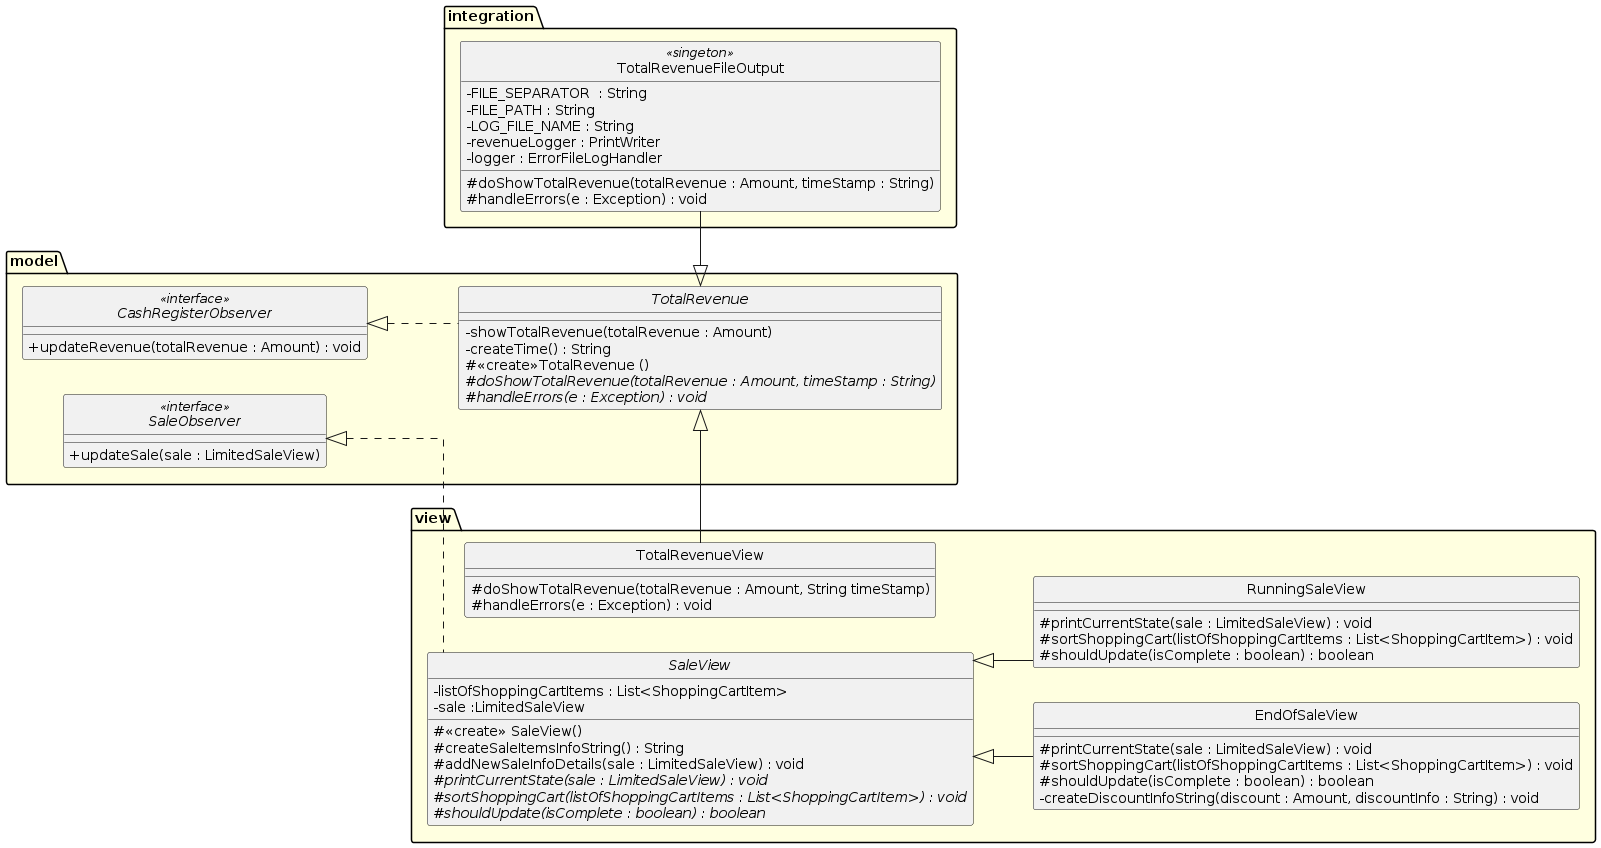
\includegraphics[width=\textwidth]{../../uml/output/uml_adp_tasks}
%        \includegraphics[trim=0cm 0cm 0cm 0cm, clip, width=\textwidth]{uml/output/uml_v3.png}
%        \caption{The Start Up \verb|Main| system operations}
        \caption{The template method applied with the observer pattern.
        This UML is an extract from the main class diagram.\\}
        \label{fig:the-observers}
    \end{center}
\end{figure}

The abstract class
\mintinline{java}{SaleView} is the template
for sale observers\footnote{The observers are only exposed to certain methods or attributes.
For example, a limited view of a particular sale is sent to the
sale observers by using an ''observered-interface'' called
\mintinline{java}{LimitedSaleView}.
This interface is implemented by the wrapper class
\mintinline{java}{LimitedSaleViewWrapper} that
only exposes certain Sale methods.}
\mintinline{java}{RunningSaleView} and
\mintinline{java}{EndOfSaleView},
while the abstract class
\mintinline{java}{TotalRevenue}
acts as the template for cash register observers
\mintinline{java}{TotalRevenueView} and
\mintinline{java}{TotalRevenueFileOutput}.
The class diagram for the observer and template method pattern
is illustrated in figure ~\ref{fig:the-observers}.

The protected abstract methods are the only methods that the subclasses \emph{must} override.
Those are
\mintinline{java}{doShowTotalRevenue(Amount totalRevenue, String timeStamp)}
\mintinline{java}{handleErrors(Exception e)}.
The former is a method that should show the total revenue and the latter should handle errors that are thrown.
In other words, the only behaviour that may vary.
Both Cash-Register observers display the total revenue and a time stamp.
The creation of the time stamp
\mintinline{java}{createTime}, and the try catch statement in
\mintinline{java}{showTotalRevenue} are joint steps
that are pulled up to the template base class.

The constructor is considered a hook method that \emph{may} be override
(for example, \mintinline{java}{TotalRevenueView} has but
\mintinline{java}{TotalRevenueView} has not).

As mentioned above, the template method
is not only applied on the task at hand (revenue updates),
but also for the observers that display sale details.
The display of sale details is updated each time an item is added to the shopping cart
and during end-of-sale performed in order to display possible discounts.
The display of the total revenue, including revenue logging to a file, is updated
each time a sale is paid for.
The outcome of refactoring to both the observer-pattern and template method
is demonstrated in all samples that are included in the README file,
and therefore presented on the GitHub repository page.

\section*{Task 2, Inheritance vs Composition}
Both inheritance and composition can be used to extend or wrap functionality
of existing classes.
Inheritance allows one to create a subtype
that can be used anywhere the superclass is expected,
while composition allows you to control how you expose the wrapped functionality,
and can also enable wrapping multiple objects or changing the wrapped object at runtime.

The class
\mintinline{java}{LoggingRandomAsRandom} extends
Random and overrides the
nextInt method to log whenever a new random number is generated.
So does the quite silly example
\mintinline{java}{LoggingRandomDiceNumbersISARandom}.


\mintinline{java}{LoggingRandomHasRandom} wraps a
Random instance and logs whenever a new number is generated.
Its silly equivalent,
\mintinline{java}{LoggingRandomDiceNumbersISARandom}.

As seen in the examples above,
both inheritance and composition can be used to extend or
wrap functionality of existing classes.
Inheritance allows you to create a subtype that can be
used anywhere the superclass is expected,
while composition allows you to control how you expose the
wrapped functionality,
and can also enable wrapping multiple objects or changing the
wrapped object at runtime.

\begin{longlisting}
    \inputminted[
        label=Random adapted with Inheritance,
        linenos=true,
        bgcolor=lightgray,
        firstline=5,
        lastline=12,
%        frame=single,
        fontsize=\footnotesize,
    ]{java}{../../additional/task2/LoggingRandomAsRandom.java}
    \caption{Random adapted with inheritance. This class generates integers and prints them to System.out}
    \label{listing:isa-a}
\end{longlisting}
\begin{longlisting}
    \inputminted[
        label=The Silly Inheritance examples,
        linenos=true,
        bgcolor=lightgray,
        firstline=5,
        lastline=12,
%        frame=single,
        fontsize=\footnotesize,
    ]{java}{../../additional/task2/LoggingRandomDiceNumbersISARandom.java}
    \caption{If random only was able to generate numbers on a dice. Here implemented with inheritance.}
    \label{listing:silly-isa-a}
\end{longlisting}

\begin{longlisting}
    \inputminted[
        label=Random adapted with Inheritance,
        linenos=true,
        bgcolor=lightgray,
        firstline=5,
        lastline=13,
%        frame=single,
        fontsize=\footnotesize,
    ]{java}{../../additional/task2/LoggingRandomHasRandom.java}
    \caption{Random adapted with Composition. This class generates integers and prints them to System.out}
    \label{listing:has-a}
\end{longlisting}
\begin{longlisting}
    \inputminted[
        label=The Silly Composite examples,
        linenos=true,
        bgcolor=lightgray,
        firstline=5,
        lastline=13,
%        frame=single,
        fontsize=\footnotesize,
    ]{java}{../../additional/task2/LoggingRandomDiceNumbersHasRandom.java}
    \caption{If random only was able to generate numbers on a dice.
    Here implemented with composition}
    \label{listing:silly-has-a}
\end{longlisting}

\section*{Task 3, Testing Output}

%\begin{longlisting}
%    \inputminted[
%        label=The common Discount-Strategy Interface,
%        linenos=true,
%        bgcolor=lightgray,
%        firstline=11,
%        lastline=21,
%%        frame=single,
%        fontsize=\footnotesize,
%    ]{java}{../../src/main/se/kth/iv1350/integration/pricing/DiscountStrategy.java}
%    \caption{Discount strategy defining the ability to calculate total price.
%        This interface shall be implemented by a class providing a promotion or
%        discount algorithm.}
%    \label{listing:discount-strategy}
%\end{longlisting}

\chapter{Discussion}
\label{sec:discussion}
\section*{The Template Model}
The Template Method Pattern is a design pattern that defines the skeleton of an algorithm in the base class but lets the extended classes override specific steps of the algorithm without changing its structure.
Here's a summary of what makes the Template Method Pattern useful:
\begin{enumerate}
    \item Code Reuse -- eliminates duplicated code.
    \item Consistency is assured since the identical steps of an algorithm are laid out in a single place (the template method in the parent class), ensuring that all implementations of the algorithm will behave consistently.
    \item By keeping the high-level algorithm in the base class and giving subclasses only the ability to change certain details, you you can prevent subclasses from making radical changes to the algorithm or its resulting behavior.
\end{enumerate}
The refactoring of the Sale Observers to utilize the Template method proved to be particularly beneficial.
There, more steps were added to the base template class than for the Cash Register Observers.

\section*{Inheritance vs Composition}
In GoF one can read that there's a principle in object-oriented design known as the
\emph{''composition over inheritance''-principle}.
This principle suggests that it can be better to achieve code reuse and flexibility by composing objects—i.e., by having instances of other classes as members of your class—rather than inheriting from a parent class.

\subsubsection*{The IS-A relationship}
When
\mintinline{java}{LoggingRandomAsRandom} extends Random, it forms an ''is-a'' relationship.
This means
\mintinline{java}{LoggingRandomAsRandom} is a Random.
It has all the methods that Random has, and any methods we add or override.
The problem comes when Random has a method that we don't want LoggingRandomAsRandom to have, or if Random changes in a future Java version in a way that breaks our class.

\subsubsection*{The HAS-A relationship}
When we use composition to create
\mintinline{java}{LoggingRandomHasRandom}, we form a ''has-a'' relationship.
\mintinline{java}{LoggingRandomHasRandom} isn't a Random, it has a Random.
It only exposes the methods we choose to expose, and it doesn't have to have any methods that don't make sense for it.
We can control how the Random's methods are used, or even use methods from multiple objects.

While inheritance can be simpler and more straightforward for simple cases, composition can provide more flexibility, better encapsulation, and make your code more resilient to changes in the classes you're reusing code from.
This is most probably why composition is often preferred over inheritance.

%\appendix
%\chapter{UML -- The Refined Design}
%\subsection*{System Operations}
%\subsubsection*{The Start up, Main System Operation}
%\begin{figure}[H]
%    \begin{center}
%        \includegraphics[width=\textwidth]{../../uml/output/uml_v3_004}
%%        \includegraphics[trim=0cm 0cm 0cm 0cm, clip, width=\textwidth]{uml/output/uml_v3.png}
%%        \caption{The Start Up \verb|Main| system operations}
%        \caption{The Main System operation}
%        \label{fig:start-up}
%    \end{center}
%\end{figure}
%

\listoflistings % Now typeset the list
\printbibliography
%med natbib
%\bibliographystyle{unsrtnat} % referenser vancouver
\end{document}
